\section{Summary} % (fold)

This dissertation has presented poolcasting, an intelligent technique that automatically programmes songs for a music channel customised for the actual audience.
The goal of poolcasting is to satisfy at once a whole group of listeners, delivering a musical sequence that matches their preferences and is at the same time varied and musically smooth.

\subsection{The goals of poolcasting} % (fold)

The novelty of poolcasting is the ability to autonomously perform a task commonly delegated to disc jockeys: to select in real time which songs to play according to the preferences of a group whose composition changes over time.
Specifically, poolcasting compiles music programmes that fulfil four properties:
\begin{enumerate}
 \item \emph{Variety}: no song or artist is repeated within a short period of time;
 \item \emph{Smoothness}: songs follow a sequence perceived as musically smooth;
 \item \emph{Customisation}: songs match the musical interests of the current audience; and
 \item \emph{Fairness}: in the long run, every listener has a similar degree of  satisfaction with respect to the music experienced.
\end{enumerate}


\subsection{The CBR process} % (fold)

The approach of poolcasting to build a group-customised musical sequence is by means of an iterated Case-Based Reasoning process that adds in real time new songs to the sequence, based on the last songs played and on the preferences of the current listeners. 
%The CBR process includes the following components.

\subsubsection{Case bases} % (fold)
The songs available to be played at any time and the preferences of the listeners for these songs constitute the case bases.
Each case is defined as a tuple <song, performing artist, individual preference>.

Individual preferences are obtained from listening habits data, analysing which songs and artists each person most played and rated in the past.
All the cases related to a listener form a \emph{case base} and describe which songs an individual would (or would not) like to hear.
The case bases of all the listeners at a given moment form the \emph{collection of case bases}.

\subsubsection{Retrieve process} % (fold)
When a new song has to be added to the musical sequence, poolcasting retrieves from the case bases a set of good candidate songs to be played next.
Songs and artists recently played are not good candidates since they do not match the requirement of variety (\ref{p:variety}).

The remaining songs are ranked according to how well they go in sequence after the last song played.
The knowledge to fulfil this task comes from the analysis of playlists collected from the Web which describe actual musical experiences of thousands of people.
From their analysis, the retrieve process determines a set of songs that are more indicate to be played after the last one and that, as such, match the requirement of smoothness (\ref{p:smoothness}).

\subsubsection{Reuse process} % (fold)
The set of retrieved candidates is then ranked according to the musical tastes of the current listeners, in order to achieve customisation (\ref{p:customisation}).
This process addresses the social choice problem of delivering content that is liked by the entire audience while preserving fairness in the long run.

In the reuse process, a set of individual preferences is extracted for each candidate song from the case bases. These preferences are then aggregated to determine the candidate song preferred by the group as a whole.
The aggregation takes place by means of a satisfaction-weighted average: songs are ranked higher if they are most liked by less satisfied listeners.
Keeping memory of past satisfactions enables the reuse process to achieve fairness (\ref{p:fairness}).

\subsubsection{Revise process} % (fold)
The ranked set of candidates is presented to the listeners who can adjust their preferences for each song.
The expressed feedback can alter the ranking of the reuse process, making a different candidate become the one with the highest group preference.

Finally, the best ranked candidate is selected and delivered to the audience.
The CBR process cycle starts again to determine the next song to add to the musical sequence.



\subsection{The Web radio application} % (fold)

To evaluate the properties of poolcasting in a real scenario, the technique has been integrated into a Web radio application to provide music channels customised for their audiences.

The result is Poolcasting Web Radio, an online radio framework that offers a \emph{social radio} experience, where the channels adapt their content for the taste of the actual audience. % and not vice versa.

The workflow of each channel follows the CBR process that characterises poolcasting.
Each channel identifies a virtual space where people find a particular subset of music (e.g., a `Rock' channel), programmed in real time according to the audience.

In this application, listeners can contribute with new songs to the repository of music by sharing their personal digital music libraries.
From each shared library, the radio parses the list of songs and the listening habits data, that is, how many times each song was played and its rating.
Analysing these data, the radio is able to assess music profiles for each channel listener.

When a new song has to be scheduled on a channel, the system first discards songs that do not fit the channel definition (e.g., non-Rock tracks) or that have been played recently.
Next, a set of good candidate songs that go well after the last song played is retrieved and ranked according to a satisfaction-weighted average of the listeners' preferences.

Using the Web interface of the radio, the audience can browse the list of ranked candidates and revise their preferences, stating explicitly positive or negative feedback for each song.
After the revision process, the best ranked candidate is finally determined as the next song to play.

% subsection poolcasting_web_radio (end)

\subsection{Evaluation} % (fold)
\label{sub:applications_evaluations}

A prototype of Poolcasting Web radio has been running in the local network of the IIIA and has served as the basis for a set of evaluations.

Ten persons have actively used the radio during one year; most of the opinions collected were positive with regard to the social radio experience.
Listeners enjoyed the fact of listening to music with friends located elsewhere and of listening to a combination of songs they already knew with songs that were unknown to them but were preferred by like-minded listeners.

Being able to discover new music was seen as a good compromise that justified the fact of being exposed, once in a while, to music outside of their interests.
Moreover, users who shared their personal libraries were able to `re-discover' songs they did not remember to have in their large collections.

A set of experiments was additionally run to evaluate the performance of poolcasting with groups made of artificial profiles with different size and musical interests.
For groups that are small or whose members have a strong musical affinity, poolcasting performs particularly well, playing musical sequences that satisfy the entire audience.

The average performance tends to decrease if the group becomes larger or musically heterogeneous since poolcasting may not always find songs that rank high in \emph{everyone}'s individual preferences. 
In these cases, poolcasting is still able to determine a musical sequence adapted for the audience, although with smaller average individual preferences.

%When the group becomes larger or musically heterogeneous, the average performance of poolcasting tends to decrease. 
%The reason is that songs that satisfy all or most of the audience, when it is large or heterogeneous, will tend to have lower average preferences.
%In these cases poolcasting is still able to determine a musical sequence adapted to the audience, although the individual preference for each song, on average, will tend to decrease.


Under every condition, poolcasting is able to fulfil the goal of fairness, selecting songs that, in the long run, satisfy the entire public.
Even when the audience is split in two discording groups (e.g., three members love the music that two members dislike and vice versa), poolcasting is able to maintain a good balance among all the participants, playing over time songs that both sub-groups like.

These positive results are due to the satisfaction-weighted aggregation method introduced in Sect.~\ref{sec:social-choice-problem} to combine multiple individual preferences into an iterated collective choice.
This method boosts the influence of less satisfied listeners, so that their favourite songs are played within a certain amount of time even if their interests belong to a minority.

\subsection{Possible applications} % (fold)

The evaluation makes clear that poolcasting can act as a good disc jockey under certain conditions, playing music that satisfies the audience and is varied and smooth.
The technique can be used to customise online radio channels (as in Poolcasting Web radio), but may also be applied to other contexts.

One possible application is to automate the selection of music in a house-party.
In the past, party guests would sometimes bring their own vinyl or compact discs to contribute to the music played.
Nowadays, most people store their music in digital devices such as iPods.
The idea of a `poolcasting party' is to set up a party where friends bring their own iPods and connect them to a personal computer, from where music will be played.
The computer runs a poolcasting system which reads the songs available on each player and autonomously generates a customised musical sequence of these songs, combining individual preferences and musical continuity. 
Similarly to a radio channel, the audience could restrict the music played to a specific subset (e.g., Dance music from the Nineties). % that best fits the spirit of the party.
As people join or leave the venue, the available music would change, and poolcasting would dynamically adapt the songs played to the current audience.

A different application for poolcasting would be to help music labels promote new releases. 
Music promotion on AM/FM radio is a common marketing strategy: labels pay radio stations to broadcast their latest songs, where the larger the audience of a station the higher the amount paid.
The problem with this strategy is that it only works for mainstream music and is not profitable for small niches of public.
With a Poolcasting Web radio, the definition of each channel would be left in the hands of the audience, according to their favourite genres, periods, tags.
In this scenario, music labels would have it easier to identify very specific niches of audience that might be interested in their upcoming releases. 
A promotion strategy for this ``long tail'' \cite{Anderson04} of listeners would be cheaper and more effective than one run on a mainstream station.

%Other scenarios where poolcasting can be applied are public spaces where people wish to listen to music in group. 
%Poolcasting would offer the dynamic of a `game' in which multiple participants can help each other discover new music they like.


\section{Contributions} % (fold)

The research reported in this dissertation offers relevant contributions to different areas: Web data mining, Case-Based Reasoning, social choice and Internet radios.

\subsection{Experiential data from the Web} % (fold)

The first contribution of this thesis is the demonstration of how experiential data collected from the Internet can be reused to perform a specific task.

Poolcasting is designed to generate `good' musical sequences and this requires domain knowledge about songs and artists that go well together in sequence.
Other researchers have proposed to extract this knowledge from the \emph{content} of musical objects, analysing their acoustic features, chords or lyrics. 
These approaches are not quite scalable since they require either the audio content, the lyrics or a symbolic representation of each song.
Moreover, these techniques can only identify songs that `sound similar', which do not necessarily correspond to songs that go well in sequence for a particular context or group.

One goal of this research was to show how the same task is better solved observing the way in which people have \emph{experienced} music in the past, to determine which songs may play well together in new sequences.
For this purpose, about a million playlists were collected from the Web, records of the way in which people organise music for their daily activities.

The analysis of co-occurrences in these playlists has resulted in the definition of a musical association degree that allows to determine which songs and artists are more `socially' associated.

The comparison of this association measure with other measures of similarity offered by popular music-related Web pages (Yahoo! Music, MusicStrands, All Music, Last.fm) has demonstrated that this approach is not only able to obtain equivalent results, but also to uncover relationships motivated by social or cultural reasons, rather than by acoustic ones.

Employing Web data mining to address problems that are typically solved by content-based techniques looks like a practical and effective approach, motivated by the fact that human experiences in multiple domains are becoming more and more available on the Internet.

\subsection{Reinterpretation of CBR} % (fold)
\label{sec:reinterpretation_of_cbr}

The second contribution of this dissertation is the reinterpretation of the Case-Based Reasoning process and its application to a dynamic group-based scenario.

The CBR process that runs poolcasting has different innovative features.
CBR has been classically understood in a single-agent framework, with \emph{individual} past experiences stored as cases to solve new tasks.
In poolcasting, past experience is obtained from \emph{multiple} people by means of playlists and listening habits.
Moreover, cases are not structured as (problem $\rightarrow$ solution) pairs, but contain the appropriate knowledge to solve the current task, that is, to determine which song to play next.

Rather than a single case base, poolcasting exploits a collection of case bases that is updated at every iteration to consider only the listeners connected at each moment.
%
The retrieve process has been reinterpreted to determine the \emph{most indicated} candidates to be played at a given time, according to the experiential knowledge extracted from playlists.
%
The reuse process attacks the social choice problem of identifying the songs preferred by the group as a whole.
%The computational cost of the reuse process is small as it focuses only on a small subset of candidate songs returned by the retrieve process.
%
The revise process updates the preferences of the audience and enables listeners to influence in real time the ranking of the retrieved set, determining which song will be played next.

One advantage of the CBR approach is that the four properties of variety, smoothness, customisation and fairness can be targeted in successive steps.
First, poolcasting looks for candidates that address sequence-related properties appropriate for \emph{every} type of audience (avoiding repetitions and jolting musical transitions).
Then, poolcasting adapts the retrieved set to a \emph{particular} audience.
In this way, the influence of the listeners is limited to a specific range of `good' songs that are indicate to be played in sequence.

A consequence of this approach is that, in the revise process, participants are requested to send feedback only for a small set of songs (the retrieved set), and not for the entire repository of music.
This encourages people to revise their preferences; showing too many options would probably obtain the opposite effect.

Another advantage of CBR is that poolcasting can both work with `passive' listeners, who never express feedback for the proposed songs, and with `active' listeners.
In the former case, models of musical preferences generated from the analysis of listening behaviour data are used to assess the preferences of the audience.
In the latter case, the adjustments made by the listeners to their music profiles enable poolcasting to learn more precisely the interests of the audience and to improve customisation over time.

Having a collection of case bases, one for each participant, is also an advantage.
Whenever people listen to music in groups, members of the audience can join or leave at different moments. At each moment, the music should be customised only for the current members.
In poolcasting, every time the CBR process is iterated, only the case bases of the current participants are considered, so that the right group-customisation is achieved. When the CBR process restarts to select the following song and the composition of the audience has changed, the collection of case bases is updated accordingly.

The characteristic of Case-Based Reasoning is to reuse past experiences to solve new tasks.
Poolcasting opens a path to apply this idea to scenarios larger than a single agent, where experience is provided by a multitude of persons (as happens on the Web) and solutions are automatically adapted to the actual preferences or needs of specific users.


\subsection{Iterated social choice} % (fold)
\label{sec:iterated_social_choice}

The third contribution of this thesis is the development of a strategy to iteratively aggregate multiple individual preferences in order to satisfy a group as a whole.

Poolcasting is faced with a series of consecutive decisions about which song to play at each moment.
These decisions cannot be taken independently since the objective is to form a globally good sequence.
The preferences of \emph{all} the participants should be considered but, at the same time, those who have not recently listened to any favourite song should be promoted, to guarantee a balance among the entire audience.

For this purpose, a novel preference aggregation method has been introduced that determines which song to select at each moment, keeping \emph{memory} of previous decisions.

The satisfaction-weighted preference aggregation consists of calculating the average of all the individual preferences, weighted according to the measure in which each person has enjoyed the experience so far.
People who have not recently listened to any of their preferred songs obtain a larger weight and vice versa.
%
Every time a new song is played, the weights are updated, which ensures, after a certain number of iterations, a fair and balanced satisfaction.

The rationale of this technique is that whenever people are exposed to content they do not particularly appreciate, they are soon after \emph{rewarded} by some of their favourite music.
This strategy is % Pareto efficient and 
a trade-off between an egalitarian and an utilitarian system.
The technique also includes a misery threshold which ensures that participants are never presented with songs they intensely dislike.

The satisfaction-weighted strategy is applicable to every domain where a \emph{sequence of inter-dependent decisions} has to be taken for a group of people.
Groups who meet on a regular basis to perform an activity together (watching movies, visiting places, attending restaurants, etc.) may use an adapted version of the strategy presented here for iterated social choice.

%Most CBR processes look for a \emph{single} optimal solution for a given individual (e.g., the best cure for a cancer patient).
%The `problem' for poolcasting is instead to build a globally good \emph{sequence} of songs over a period time, targeting a group whose composition can change over time.
%This task is approached pursuing a trade-off between desirable musical properties (variety, smoothness) and audience satisfaction (customisation, fairness).



% section iterated_social_choice (end)


\subsection{A social radio experience} % (fold)
\label{sub:a_social_radio_experience}

The fourth contribution of this thesis is the development of an online application to provide group-customised music channels.

Online radios stream millions of music channels that are not affected by who is actually listening. 
Poolcasting Web radio takes instead advantage of the social nature of the Internet to stream music channels customised for their audience.

Customised music streams are typical of digital music services such as Last.fm and Pandora which provide \emph{private} music channels, personalised for \emph{individuals}.
The innovation of Poolcasting Web radio is to offer % for the first time
\emph{public} radio channels that anyone can join at any moment, where the content is adapted to a \emph{group} of listeners in real time.

Poolcasting Web radio also offers innovative features to increase the social nature of the experience: listeners can vote for the proposed songs, can create new channels and, most importantly, can share their personal music libraries, contributing with music to the collection of songs broadcast on the radio.
%
According to a recent study \cite{McGuire05}, nearly one-fourth of frequent online music users say the ability to share music with others in some fashion is an important criterion when selecting an online music service.

Poolcasting Web radio combines bottom-up and top-down approaches: users can express their musical preferences while the actual choice of music played is taken by a CBR process that iteratively checks which songs are available and who is listening and selects the song most likely to satisfy the current audience.

With Poolcasting Web radio, the social component that characterises many real-world situations is integrated for the first time into a Web application.
Listeners can influence the music played, chat with each other within a channel, define new channels and share personal libraries and listening habits.

Friends located around the world can meet in a virtual space created ad hoc for their musical interests and share a listening experience that is not offered by other Web services and which allows to easily get to share and discover music.

% subsection a_social_radio_experience (end)


\section{Future work} % (fold)


% section future_work (end)

Although this dissertation has focused on customising \emph{musical} content for a group of listeners, the techniques presented can be extended to  content of different nature.
The idea of `poolcasting' comes from the words:
%\begin{itemize}
%	\item \textbf{pool}: a combination of resources, funds, etc., for common advantage; and
%	\item \textbf{cast}: to send forth, to deliver.
%\end{itemize}
\begin{quote}
pool (noun) --- a combination of resources, funds, etc., for common advantage; and

cast (verb) --- to send forth, to deliver;
\end{quote}
and can be defined as follows:
\begin{quote}
\textbf{poolcast} (verb)  --- to collect knowledge about resources and people, and use such knowledge to deliver the right sequence of resources for the common advantage of a group of people.
\end{quote}

\begin{figure}[bthp]
\centering \setlength{\abovecaptionskip}{3pt}
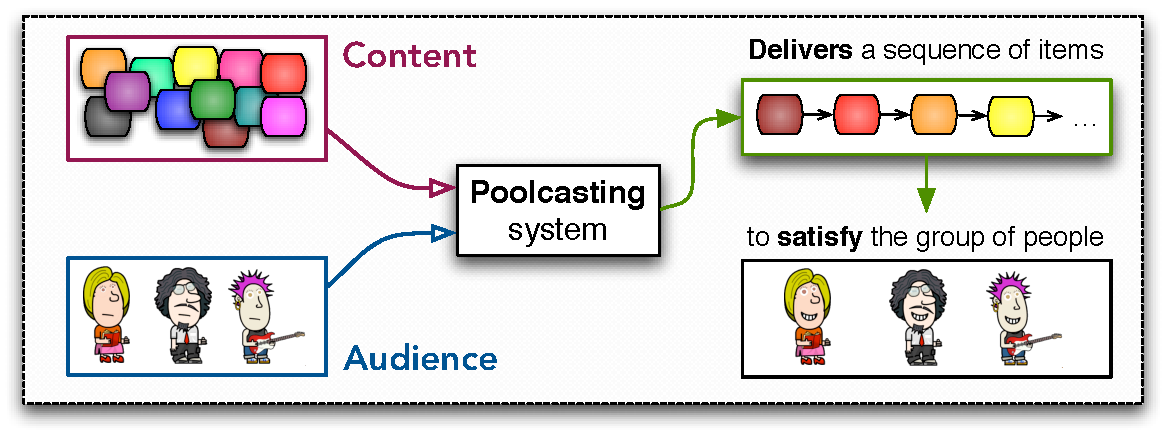
\epsfig{file=img/fig7_1, width=\textwidth}
\caption{A poolcasting system scenario.}
\label{fig:poolcasting-scenario}
\end{figure}

Poolcasting identifies a process that does not require human intervention and works sequentially, %(Fig.~\ref{fig:poolcasting_loop_channel}), 
selecting which items to deliver to the audience based on the previous items and on the preference and satisfaction of the audience.
Poolcasting can be considered, similarly to collaborative filtering, as a family of techniques applicable to user-adaptive systems.
%\begin{figure}[tbhp]
%\centering \setlength{\abovecaptionskip}{3pt}
%\epsfig{file=img/poolcasting_loop_channel2, width=\textwidth}
%\caption{The iterative process of a poolcasting channel.}
%\label{fig:poolcasting_loop_channel}
%\end{figure}

This dissertation has shown that reusing experiences collected from the Web to provide group-customised channels is a practical and productive research path.
Future work will be dedicated to investigate domains other than music where this approach can result effective.

\subsection{Generalising poolcasting} % (fold)
\label{sec:generalisation}

To extend poolcasting to other domains, it is important to summarise the fundamental features and requirements of the presented technique.

The first characteristic of poolcasting is its \emph{iterative} nature.
The goal of the technique is to generate a good \emph{sequence} of items\,---\,not just one\,---\,and for this reason a selection process is iterated multiple times.
At each iteration, poolcasting holds \emph{memory} of the previous selections to ensure that the whole sequence fulfils the desired requirements.

The second property of poolcasting is its \emph{social} nature.
The technique adapts content to a group\,---\,not an individual.
When members of a group have different preferences, poolcasting pursues fairness with a sequence that can possibly satisfy everyone at the same degree.
Poolcasting is designed for intentional groups, who accept to collaborate rather than to compete, for whatever reason that keeps the group alive.
The composition of the group can change over time and members can either be co-located or displaced.

The third characteristic is that domain knowledge comes from \emph{reusing past experiences}. % under a CBR view?
The principle is that the best way to customise content for a group is to learn from the way in which others have experienced that content in the past.
In particular, the focus is on the Web which offers the largest data source for human experiences.

The last relevant property is that poolcasting does not just \emph{recommend} but actually \emph{delivers} adapted content (e.g., broadcasting music on the Web), enabling the audience to share an actual experience and express immediate feedback which is valuable to improve customisation over time. 

\subsubsection{Poolcasting in the domain of movies} % (fold)
\label{sub:poolcasting_in_the_domain_of_movies}

One scenario where poolcasting could be useful is that of a family or a group of friends who meet weekly to watch movies together.
Each individual might have different `watching habits' and enjoy more or less different genres but still long for a social experience that reunites them week after week. % in front of a screen.

In this kind of situation, people implicitly accept the social compromise that they will probably not watch only movies they know and like, but will have the chance to discover titles enjoyed by their friends.

This scenario resembles that of Poolcasting Web radio, but the extension to the domain of movies requires some adjustments.
While songs in a radio are played one right after the other, movies are watched in separate days, therefore their order and continuity is not as relevant as in the case of music.

The satisfaction decay also changes: listening to three consecutive `less preferred' songs in a radio channel may be acceptable for an individual, since they would only count for 10 minutes of an entire music programme; watching three `less preferred' movies in a row, on the other hand, would be less acceptable, since they would correspond to three weeks of negative satisfaction for a specific individual.

Another difference resides in the data collected from the Web to identify associations. Working with movies requires to gather `watch-lists', sequences of titles watched by a person within a certain period.
Similarly to music, Web communities exist that make these data available for millions of users.

The co-occurrence analysis of these data is also different.
In the case of music, the simple fact of observing two songs occurring together in playlists suggests an association between them.
In the case of movies, an association can be derived only when many people watched the same two movies and \emph{rated them} identically.

A complete development of a movie-related poolcasting system remains future work, but preliminary studies suggest that the analysis of Web-mined data can produce good lists of top associated movies, as reported in Appendix~\ref{cha:appendix}.
%, similar to the lists of top associated songs and artists presented in Sect.~\ref{sub:the_smoothness_degrees_we_obtain}.

% Other domains will also be investigated, such as automatically selecting a sequence of interesting \emph{news items} for a group of displaced friends or deciding which \emph{TV shows} to broadcast for a `family prime-time' session. % sitting in front of a TV set.

\subsubsection{Poolcasting news items} % (fold)

Another promising scenario for poolcasting is delivering news items to a group of displaced friends.
Nowadays there is a clear discrepancy in the way in which news are produced and consumed.
Newspapers, newscasts and magazines force users to experience news in a fixed order, determined by the editorial board to satisfy an imaginary `average' consumer (e.g., first politics, then economics, then weather, then sport). 
However every person has a particular way of experiencing news; for instance one might flip through the first pages of a newspapers and skip directly to sport and weather.

Applying the poolcasting strategy to news items would mean to let people organise themselves in groups (\emph{news channels}) where they would specify their interests either explicitly (by means of genres, periods, tags) or implicitly (inferred from their previous experiences).
 
Within a channel, people would share news items with others and, in return, discover news that interest other like-minded persons. News producers would benefit from this model since they would be able to deliver the right \emph{content} to the right \emph{target}. 

Poolcasting news items would also blunt geographical constraints. 
People would be able to access their own `local news' channels, independently from their actual location. 
An Indian citizen living abroad, for instance, would still be able to receive daily updates about his hometown and become aware of news items prompted by his friends in India.

\subsubsection{Poolcasting TV programmes} % (fold)

A different domain where to apply poolcasting is that of a group of people, sitting together in front of a TV set, who have to decide which programmes to watch.
Thanks to PVRs (Personal Video Recorders), viewers can nowadays \emph{personalise} the order in which they wish to experience TV shows, but 
these systems only work for one person at the time and do not allow a \emph{group} to find a sequence of programmes that can satisfy everyone.

A common situation is that of a family where the father likes sport and action/comedy movies, the mother likes comedy movies and quiz shows, the grandmother likes documentaries and talk shows, the kid likes animated series and comedies: what programmes should they watch together?
Is there a social alternative to splitting the family into four separate screens?

The idea of a `poolcasting TV' consists in a system that autonomously configures prime-time TV group sessions day after day. 
This system would first build user profiles of each spectator, based on explicit feedback and observed behaviours (e.g., which shows each person tends to watch, at which time, for how long, when is the person at home).
During each session, the system would then aggregate multiple preferences, trying to satisfy the whole family in the long run.
For instance, one night the system might first broadcast an episode of an animated series, so the kid can happily go to sleep; then a documentary about sport legends, to generate an enriching discussion between father and grandmother; then a comedy movie, which would fairly satisfy all the adults.
Memory of past choices would help achieve balance and fairness among all the family members along time.

\subsection{Improving poolcasting} % (fold)
\label{sub:improving_the_quality_of_music_channels}

A different direction for future work deals with ways to improve the experience of members of poolcasting channels.

\subsubsection{Self-adaptive channels} % (fold)

A possible improvement to poolcasting is to introduce self-adaptive channels. These channels would diagnose decreases in performance and react accordingly, suggesting a solution to the participants. 

An example is given by the situation where a Poolcasting Web radio channel is listened by two discordant groups of listeners and the system has to struggle to adapt the music for the entire audience. 
In this case, a self-adaptive channel would detect the situation and suggest the two sub-groups to split into two separate channels, in order to maintain a higher degree of group satisfaction.

Introducing self-adaptive channels would be of great advantage to the participants. 
Self-adaptive channels can be seen as form of \emph{goal-driven learning} \cite{Leake93} as they would recognise situations where some type of failure occurs, access a library of possible correcting actions and then apply the best suited one to fix the problem. 

\subsubsection{Fuzzy affinity degrees} % (fold)
\label{ssub:smooth_genre_transitions}

A different direction to improve poolcasting experience is to enrich \emph{music ontology} from simple Boolean categories to fuzzy affinity degrees.

Poolcasting can currently categorise songs and artists in the music pool only in Boolean terms. 
Madonna, for instance, \emph{belongs to} the genre Pop and \emph{not to} the genres R\&B or Jazz. Likewise, Madonna \emph{has been tagged as} `female pop' and \emph{not as} `Spanish pop'.

The limitation of this representation becomes clear when poolcasting has to schedule music for multi-genre channels, for instance for a radio channel defined as `genre in (Pop, R\&B)'.
Ideally, a good musical selection for this channel would be to first play a song from the \emph{core} of a genre (e.g., a Pop song), then a series of songs \emph{in between} two genres (e.g., Pop/R\&B tracks) to finally reach a song in the core of the second genre and gradually move back to the first genre. %, and so on.
%
%Nevertheless, poolcasting cannot build such a sequence because it lacks the concepts of `core' and `in between' songs. 
%Poolcasting only knows which songs/artists belong to either genre, but not at which degree.
%
In order to achieve this behaviour, the music ontology employed by poolcasting has to be enriched to include \emph{fuzzy membership degrees}, to measure the \emph{degree} in which each song or artist belongs to each genre or tag. % (e.g., Madonna is 0.4 Pop, 0.8 R\&B, 0.3 Jazz, and so on). 
%For example, Madonna would not be characterised as Pop and not R\&B nor Jazz, but as a vector of fuzzy membership values [Pop = 0.4, R\&B = 0.8, Jazz = 0.3].

A method to describe songs and artists in terms of fuzzy membership degrees was introduced by the author in \cite{Baccigalupo08}.
Thanks to this method, artists can be characterised as vectors of fuzzy membership values rather than simply as Boolean categories. 
The music of Madonna, for instance, can be described as belonging to different genres at different fuzzy degrees: Pop (0.4), R\&B (0.8), Jazz (0.3), and so on.

%Integrating this approach into poolcasting would enable users to better define music channels, specifying whether they would like to hear only artists from the \emph{core} of a given genre (with high membership values) or whether they expect \emph{cross-genre} transitions to occur. 

Future work will be dedicated to embody the concept of ``genre affinity degree'' into poolcasting.
Users would benefit from this approach as they would be able to specify whether 
a channel should only play \emph{core} artists of a given genre (who show a high membership degree) or whether \emph{cross-genre} artists are allowed as well.

Poolcasting could also be able to better programme multi-genre radio channels, playing music that smoothly shifts from the core of a genre, to cross-genre songs, to songs belonging to a different genre and so on.
This improvement would make poolcasting behave more similarly to professional disc jockeys, who are able to swiftly transport music from a style/genre/tempo to a different one without disrupting transitions.



% subsubsection smooth_genre_transitions (end)


% subsection improving_the_quality_of_music_channels (end)
%\subsection{Fuzzy genres?} % (fold)
%\label{sub:fuzzy_genres_}

%boh
% subsection fuzzy_genres_ (end)

% section generalisation (end)


\section{Related publications} % (fold)
\label{sec:future_work}

The following papers were published as part of this research.

\begin{itemize}
    \item[] \cite{Baccigalupo06}
    C.~Baccigalupo and E.~Plaza.
    \newblock Case-based sequential ordering of songs for playlist recommendation.
    \newblock In T.~Roth-Berghofer, M.H. G{\"o}ker, and H.A. G{\"u}venir, editors, {\em Advances in {C}ase-{B}ased {R}easoning, Proceedings of the 8th European Conference on Case-Based Reasoning (ECCBR 2006)}, volume 4106 of {\em Lecture Notes in Computer Science}, pages 286--300. Springer, 2006.

      \item[] \cite{Baccigalupo07}
      C.~Baccigalupo and E.~Plaza.
      \newblock A case-based song scheduler for group customised radio.
      \newblock In R.~Weber and M.M. Richter, editors, {\em Case-{B}ased {R}easoning Research and Development, Proceedings of the 7th International Conference on Case-Based Reasoning (ICCBR 2007)}, volume 4626 of {\em Lecture Notes in Computer Science}, pages 433--448. Springer, 2007.

      \item[] \cite{Baccigalupo07c}
      C.~Baccigalupo and E.~Plaza.
      \newblock Mining music social networks for automating social music services.
      \newblock In {\em Workshop Notes of the ECML/PKDD 2007 Workshop on Web Mining 2.0}, pages 123--134, 2007.

      \item[] \cite{Baccigalupo07e}
      C.~Baccigalupo and E.~Plaza.
      \newblock Poolcasting: A social {W}eb radio architecture for group customisation.
      \newblock   In {\em Proceedings of the Third International Conference on Automated Production of Cross Media Content for Multi-Channel Distribution (AXMEDIS '07)}, pages 115--122. IEEE Computer Society, 2007.

      \item[] \cite{Baccigalupo07f}
      C.~Baccigalupo and E.~Plaza.
      \newblock Sharing and combining listening experience: a social approach to {W}eb radio.
      \newblock   In {\em Proceedings of the 2007 International Computer Music Conference (ICMC)}, pages 228--231, 2007.

      \item[] \cite{Baccigalupo08}
      C.~Baccigalupo, E.~Plaza, and J.~Donaldson.
      \newblock Uncovering affinity of artists to multiple genres from social behaviour data.
      \newblock In ISMIR \shortcite{ISMIR08}, pages 275--280.

      \item[] \cite{Plaza09}
      E.~Plaza and C.~Baccigalupo.
      \newblock Principle and praxis in the experience {W}eb: a case study in social music.
      \newblock In S.J. Delany, editor, {\em Proceedings of the ICCBR 2009
        Workshops}, pages 55--63. University of Washington Tacoma, 2009.


\end{itemize}

% SHOULD I ADD PRESENTATIONS? ECCBR06 industry, RECSYS 06 and ESTIU 2.0 ?


% mysql> select * from _all_movies_titles where title = "Boys Don't Cry" limit 3;
% +-------+------+----------------+
% | id    | year | title          |
% +-------+------+----------------+
% | 11880 | 2000 | Boys Don't Cry |
% | 12500 | 1999 | Boys Don't Cry |
% +-------+------+----------------+
% 2 rows in set (0.02 sec)
% 
% mysql> insert into customers_boys select distinct customer_id from ratings where movie_id = 12500;
% Query OK, 48419 rows affected (20.67 sec)
% 
% mysql> insert into ratings_boy select ratings.* from ratings join customers_boy using(customer_id);
% Query OK, 21406766 rows affected (221.07 sec)
% 
% mysql> insert into ratings_boy_boy select customer_id, date, rating from ratings_boy where movie_id = 12500;
% Query OK, 48419 rows affected (2.14 sec)
% 
% mysql> insert into ratings_boy_others_5days select r.movie_id, r.customer_id, datediff(r.date, s.date) from ratings_boy r join ratings_boy_boy s on r.customer_id = s.customer_id and r.rating = s.rating and abs(datediff(r.date, s.date)) <= 5 and movie_id <> 12500;
% Query OK, 1538594 rows affected (150.85 sec)
% 
% mysql> insert into frequency_boy_others_5days select movie_id, count(customer_id) as c, count_ratings, datediff from ratings_boy_others_5days join _most_rated_movies using(movie_id) group by movie_id, datediff;
% Query OK, 51443 rows affected (13.28 sec)
% 
% mysql> insert into results_boy_others_beta_08_d06 select movie_id, sum(pow(0.6, abs(datediff))*(coratings/20569)*pow(1-(popularity/479454), 0.8)) from frequency_boy_others_5days;
% Query OK, 1 rows affected (0.08 sec)
% 
% mysql> insert into results_boy_others_beta_08_d06 select movie_id, sum(pow(0.6, abs(datediff))*(coratings/20569)*pow(1-(popularity/479454), 0.8)) from frequency_boy_others_5days group by movie_id;
% Query OK, 8111 rows affected (0.10 sec)
% 
% mysql> select title, year, t from results_boy_others_beta_08_d06 join _all_movies_titles on movie_id = id order by t desc limit 10;

% NOTA: Ora nel MySQL ho la tabella che lista per ogni coppia di film il both_rated e both_best, ma % senza la distanza e l'ordine. Quindi dovrei avere questi dati, poi spiegare come l'ordine sia meno importante nei film, dato che sono piu' lunghi.. o forse anche togliere la distanza!!! 

% Quindi lo posso fare, basta fare cosi': se X = 175 e Y = 197
%d = select both_best from movies_to_movies_after100k where movie1_id = 175 and movie2_id = 197
%cx = select both_best from movies_to_movies_after100k where movie1_id = 175 and movie2_id = 175
%cy = select both_best from movies_to_movies_after100k where movie1_id = 197 and movie2_id = 197
%s = $\frac{d^{\beta + 1}}{cx \cdot cy^\beta}$

% subsection smoothness_in_movies (end)
 
% subsection customisation (end)





% section future_work (end)